\documentclass{ieeeaccess}
\usepackage{cite}
\usepackage{amsmath,amssymb,amsfonts}
\usepackage{algorithmic}
\usepackage{graphicx}
\usepackage{textcomp}

\usepackage[ruled,noend,linesnumbered]{algorithm2e}
\usepackage{graphicx,color,psfrag}
\usepackage{amsmath}
\usepackage{amsfonts}
\usepackage{amssymb}
\usepackage{bigdelim}
\usepackage{dsfont}
\usepackage{color, soul}
\usepackage{caption}
\usepackage{subcaption}
\usepackage{url}

\def\BibTeX{{\rm B\kern-.05em{\sc i\kern-.025em b}\kern-.08em
    T\kern-.1667em\lower.7ex\hbox{E}\kern-.125emX}}
\begin{document}
\history{Date of publication xxxx 00, 0000, date of current version xxxx 00, 0000.}
\doi{10.1109/ACCESS.20xx.0000000}

\title{Visibility Aware In-Hand Object Pose Tracking in Videos with Transformers}

\author{\uppercase{Phan Xuan Tan}\authorrefmark{1},
\uppercase{Dinh-Cuong Hoang}\authorrefmark{2},
\uppercase{Eiji Kamioka}\authorrefmark{1},
\uppercase{Anh-Nhat Nguyen}\authorrefmark{3},
\uppercase{Duc-Thanh Tran}\authorrefmark{3}
\uppercase{Van-Hiep Duong}\authorrefmark{3},
\uppercase{Anh-Truong Mai}\authorrefmark{3},
\uppercase{Duc-Long Pham}\authorrefmark{3},
\uppercase{Khanh-Toan Phan}\authorrefmark{3},
\uppercase{Xuan-Tung Dinh}\authorrefmark{3},
\uppercase{Tran Thi Thuy Trang}\authorrefmark{3},
\uppercase{Xuan-Duong Pham}\authorrefmark{3},
\uppercase{Nhat-Linh Nguyen}\authorrefmark{3},
\uppercase{Viet-Anh Trinh}\authorrefmark{2},
\uppercase{Khanh-Duong Tran}\authorrefmark{2}, and
\uppercase{Son-Anh Bui}\authorrefmark{2}}

\address[1]{College of Engineering, Shibaura Institute of Technology, Tokyo 135-8548, Japan}
\address[2]{Greenwich Vietnam, FPT University, Hanoi, 10000, Vietnam}
\address[3]{IT Department, FPT University, Hanoi, 10000, Vietnam}

%\tfootnote{This paragraph of the first footnote will contain support
%information, including sponsor and financial support acknowledgment. For
%example, ``This work was supported in part by the U.S. Department of
%Commerce under Grant BS123456.''}

\markboth
{P. X. Tan \headeretal: In-Hand Object Pose Tracking}
{P. X. Tan \headeretal: In-Hand Object Pose Tracking}

\corresp{Corresponding author: Dinh-Cuong Hoang (e-mail: cuonghd12@fe.edu.vn).}


\begin{abstract}

In-hand object pose estimation is essential in various engineering applications, such as quality inspection, reverse engineering, and automated manufacturing processes. However, achieving accurate pose estimation becomes difficult when objects are heavily occluded by the hand or blurred due to motion. To address these challenges, we propose a novel framework that leverages the power of transformers for spatial-temporal reasoning across video sequences. Our approach utilizes transformers to capture both spatial relationships within each frame and temporal dependencies across consecutive frames, allowing the model to aggregate information over time and improve pose predictions. A key innovation of our framework is the introduction of a visibility-aware module, which dynamically adjusts pose estimates based on the object's visibility. This module utilizes temporally-aware features extracted by the transformers, allowing the model to aggregate pose information across multiple frames. By integrating this aggregated information, the model can maintain high accuracy even when portions of the object are not visible in certain frames. This capability is particularly crucial in dynamic environments where the object's appearance can change rapidly due to hand movements or interactions with other objects. Extensive experiments demonstrate that our method significantly outperforms state-of-the-art techniques, achieving a 6\% improvement in overall accuracy and over 11\% better performance in handling occlusions.

\end{abstract}

\begin{keywords}
Pose estimation, robot vision systems , intelligent systems,   deep learning, supervised learning, machine vision.
\end{keywords}

\titlepgskip=-21pt

\maketitle

%%%%%%%%%%%%%%%%%%%%%%%%%%%%%%%%%%%%%%%%%%%%%%%%%%%%%%%%%%%%%%%%%%%%

\input{Introduction} 
%
\section{Related Work}
\label{sec:Related}

\subsection{Object Pose Estimation from a Single Image}

Vision-based object pose estimation involves detecting an object of interest and estimating its 6-DoF (Degrees of Freedom) pose, which includes 3D rotation $\mathbf{R} \in SO(3)$ and 3D translation $\mathbf{t} \in \mathbb{R}^3$, relative to a canonical frame. The assumption is that the CAD model of the object is available beforehand. Depending on the input data format, object pose estimation methods can be classified into three categories: depth-based methods \cite{wang20216d, gao20206d, guo2021efficient}, RGB-based methods \cite{billings2019silhonet, peng2019pvnet, wang2021gdr}, and RGBD-based methods \cite{wang2019densefusion, he2020pvn3d, hong2024rdpn6d}. Depth-based and RGBD-based methods rely on depth images captured by depth cameras, which limits their applicability in certain scenarios, as depth cameras are not widely used in many applications. In contrast, RGB-based methods require only a single RGB image, making them more practical and accessible for real-world use. However, the challenge of estimating the 3D pose from a single RGB image stems from the loss of depth information and ambiguities in perspective projection.

Traditional methods \cite{lowe1999object, lepetit2005monocular} approached this problem by establishing correspondences between 2D image features and 3D points on the object model. These approaches rely on handcrafted features, but they are susceptible to image variations, background clutter, and occlusions. The advent of deep learning has shifted the focus towards learning-based methods, which have demonstrated superior performance by leveraging large datasets and powerful convolutional neural networks (CNNs). Deep learning-based methods for object pose estimation can be broadly categorized into three classes: direct methods \cite{xiang2017posecnn, kehl2017ssd, trabelsi2021pose, wang2021gdr}, keypoint-based methods \cite{rad2017bb8, tekin2018real, oberweger2018making, peng2019pvnet}, and dense coordinate-based methods \cite{li2019cdpn, park2019pix2pose, zakharov2019dpod}. Direct methods treat pose estimation as a regression or classification task, directly predicting pose parameters from input images \cite{xiang2017posecnn, kehl2017ssd, trabelsi2021pose}. While these methods are intuitive, they often require additional time-consuming pose refinement operations to improve accuracy. To address these limitations, other approaches \cite{hu2020single, chen2020end, wang2021gdr} have modified indirect methods into direct methods by leveraging neural networks to establish 2D-3D correspondences, followed by solving the Perspective-n-Point (PnP) problem \cite{lepetit2009ep} within a deep learning framework. These methods, although more efficient, often underperform compared to other approaches due to their reliance on deep networks alone to recover the full 6-DoF parameters. In contrast to directly predicting pose-related parameters, correspondence-based methods, such as keypoint-based methods \cite{rad2017bb8, tekin2018real, oberweger2018making, peng2019pvnet}, have shown superior performance by building 2D-3D correspondences. Keypoint-based methods utilize CNNs to detect 2D keypoints in the image, followed by solving the PnP problem to estimate the object's pose \cite{lepetit2009ep}. These methods achieve notable success, but they require predefined keypoints for each object, leading to high labor costs. Beyond keypoint-based methods, dense coordinate-based methods \cite{li2019cdpn, park2019pix2pose, zakharov2019dpod} represent another class of correspondence-based approaches. These methods frame the 6-DoF pose estimation task as building dense 2D-3D correspondences, followed by a PnP solver to estimate the object's pose. Dense correspondences are obtained by predicting 3D object coordinates for each object pixel or by generating dense UV maps. However, predicting object coordinates for dense correspondences is more challenging than detecting sparse keypoints due to the larger search space involved.

Despite the recent progress, object pose estimation from a single image remains a difficult and unsolved problem, particularly in scenarios involving heavy occlusion or rapid motion, such as hand-held objects. To address these challenges, our proposed method leverages a sequence of images rather than a single image to estimate the in-hand object pose, which improves robustness and accuracy in dynamic environments.

\subsection{Deep Learning-based Object Pose Tracking}

Object pose tracking extends the problem of pose estimation to a temporal sequence of images, where the goal is to maintain an accurate estimate of an object's 3D pose across a video sequence \cite{sun2021robust, huang2021pixel, stoiber2020sparse, tian2022large}. Deep learning-based methods for object pose tracking are generally classified into two categories: tracking by refinement \cite{garon2017deep, marougkas2020track, manhardt2018deep, li2018deepim, dosovitskiy2015flownet, wen2020se} and tracking by optimization \cite{deng2021poserbpf, majcher20203d, zhong2020seeing, wang2023deep}.

Tracking by refinement methods initialize the object's pose in each frame using the pose estimate from the previous frame and then refine it based on the new input. Garon et al. \cite{garon2017deep} pioneered this approach by using the pose from the last frame to render a synthetic RGB-D frame of the target object. Their network then takes the rendered image and the observed image as inputs to predict the relative 6-DoF pose between these frames. To improve performance in cluttered and occluded environments, Marougkas et al. \cite{marougkas2020track} introduced multiple parallel soft spatial attention modules into the network architecture. While the above methods rely on RGB-D data, Manhardt et al. \cite{manhardt2018deep} proposed a refinement approach that works solely with RGB images. They introduced a new visual loss function that drives the pose update process by aligning object contours in the image, avoiding the need for explicit appearance models or depth data. These refinement methods typically utilize the pose from the last frame as an initialization for the current frame, refining it through a single forward pass in a neural network. However, this process can lead to coarse pose predictions due to the limited refinement performed. To address this, DeepIM \cite{li2018deepim} was introduced as a method for iterative refinement. In DeepIM, the network iteratively matches the rendered image against the observed image, predicting the relative pose between the two using a FlowNet-like architecture \cite{dosovitskiy2015flownet}. Although DeepIM demonstrates strong performance, it requires extensive training on real-world images and suffers from slow runtime during inference. Wen et al. \cite{wen2020se}, on the other hand, achieves real-time performance by training solely on synthetic data. Its success is attributed to techniques such as rotation-translation disentanglement, the Lie algebra representation of rotation, and DR data enhancement. While tracking by refinement methods generally achieve high accuracy, they depend on rendering CAD models into synthetic images, which is often non-differentiable, hindering end-to-end training. Additionally, the quality of the rendering and the CAD models themselves can significantly impact tracking performance. 

In contrast to refinement-based methods, tracking by optimization focuses on formulating the pose tracking problem as an optimization task. PoseRBPF \cite{deng2021poserbpf} exemplifies this approach by combining Rao-Blackwellized particle filtering with a learned autoencoder network for pose updates. In this framework, the particle filter estimates discretized distributions over rotations and translations, with translations updated directly by the filter. Rotations are updated by comparing image descriptors with precomputed entries in a codebook generated by the autoencoder. While PoseRBPF performs well, it requires discretization of the continuous rotation space to build the codebook, which limits its performance and increases the algorithm's time complexity as the number of discretized rotations grows. Majcher et al. \cite{majcher20203d} also utilize particle filtering in their tracking framework. In their approach, a U-Net is used to segment the target object in advance, and the object's 6-DoF pose in the current frame is estimated by matching the segmented object with a rendered image based on the pose from the last frame. The final pose is obtained by optimizing the difference between object silhouettes and edges, with the particle filter estimating the posterior probability distribution. Zhong et al. \cite{zhong2020seeing} introduced a method that integrates a learning-based video segmentation module into an optimization-based pose estimation pipeline. Wang et al. \cite{wang2023deep} introduced a three-phase pipeline for object pose tracking. The process begins with an FPN-Lite network integrated with MobileNetV2 to extract multi-level features from the current image and to project a 3D object model for deriving 2D contours based on the pose from the previous frame. Next, a boundary prediction network is employed, which takes features from local regions around the contours as input and outputs a probability distribution representing the true boundary locations. Finally, the 6-DoF object pose is refined using Newton's method, leveraging the boundary probability distribution. The primary advantage of tracking by optimization methods lies in their interpretability. However, the optimization process is typically slow, and challenges such as occlusion remain problematic for many methods in this category.

\subsection{Transformer-based Methods}

The Transformer model \cite{vaswani2017attention} has emerged as the dominant architecture for a wide range of natural language processing (NLP) tasks. Unlike CNNs, which rely on strong inductive biases, the Transformer's self-attention mechanism is highly adaptable, allowing it to focus on different parts of a sequence of features. Transformer-based methods have recently been introduced to the field of computer vision, offering a powerful alternative to traditional CNNs. The Vision Transformer (ViT) \cite{dosovitskiy2020image} is a direct adaptation of the transformer architecture to image processing. Instead of using convolutional layers, ViTs divide an image into fixed-size patches, linearly embed each patch into a vector, and then apply the transformer architecture to these vectors. Self-attention allows the model to capture global dependencies and relationships between different parts of the image, which can be beneficial for tasks like image classification and object detection. Some approaches combine traditional convolutional neural networks (CNNs) with transformers \cite{liu2021swin, guo2022cmt}. Hybrid models use CNNs to extract initial features from images and then apply self-attention mechanisms to these features. This hybrid approach leverages the strengths of both architectures: the locality and efficiency of CNNs and the global context understanding of transformers. In this work, we also emplopy a hybrid model. While transformer-based methods are still relatively new in the domain of object pose estimation and tracking, they represent a promising direction for future research. Their ability to model global context and capture intricate relationships within the data makes them well-suited for advancing the state of the art in both single-image pose estimation and pose tracking.

%
\section{Method}

\begin{figure*}[h!]
	\centering
	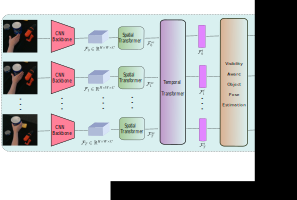
\includegraphics[width=0.98\linewidth]{figs/overview}
	\caption{Overview of the proposed framework for in-hand object pose tracking. Our approach leverages transformers to capture both spatial relationships within individual frames and temporal dependencies across image sequences, enabling robust frame-wise object pose estimation. To address challenges posed by heavy occlusion or motion blur, a visibility-aware module integrates temporally-aware features and aggregates pose information from neighboring frames. This allows the model to maintain accurate pose estimates even in difficult scenarios where direct visual cues are limited or absent.}
	\label{fig:overview}
\end{figure*}

The overview structure of our framework is illustrated in Figure \ref{fig:overview}. Given a sequence of RGB images $\mathcal{V} = \lbrace I_t \rbrace_{t=1}^{T}$, where $T$ represents the total number of frames, the objective is to estimate the object's 6D pose $\mathbf{P}_t = (\mathbf{R}_t, \mathbf{t}_t)$ for each frame $I_t$. This pose consists of the rotation matrix $\mathbf{R}_t$ and the translation vector $\mathbf{t}_t$, which describe the rigid transformation of the object from its coordinate system to the camera coordinate system. We assume that a 3D model of the object is available, and its coordinate system is defined within the 3D space of the model. The framework first utilizes a CNN backbone (ResNet-50 with a truncated FPN) to extract spatial features \( \mathcal{F}_t \) from each frame. These features are then enhanced by a spatial transformer $\mathcal{M}_{s}$, which captures non-local dependencies within each frame to improve the modeling of complex hand-object interactions. The spatial transformer encoder produces contextually enriched features \( \mathcal{F}^s_t \), which are further processed by a temporal transformer $\mathcal{M}_{s}$ that models temporal relationships across frames. The temporal transformer outputs latent vectors \( \mathcal{F}^t_t \), which are passed through an MLP to predict the object's pose \( \hat{\mathbf{P}}_t \) for each frame. Additionally, a visibility-aware module $\mathcal{M}_{va}$ predicts the object's visibility score \( v_t \) for each frame, dynamically adjusting pose predictions based on occlusion levels. This module aggregates pose information from visible frames to support pose estimation in occluded frames using a cross-attention mechanism, ensuring robust performance under heavy occlusions and rapid motion.

\subsection{Spatial-Temporal Transformer}

\subsubsection{CNN Backbone}

Inspired by the hybrid model proposed by \cite{carion2020end}, our method begins by leveraging a truncated FPN \cite{lin2017feature} with ResNet50 \cite{he2016deep} to extract the initial in-hand object features $\mathcal{F}_t \in \mathbb{R}^{H \times W \times C}$ for each frame $I_t$. While CNNs, through their convolutional kernels, are effective at capturing local two-dimensional structures, they struggle with occlusions where local details are obscured or distorted. To mitigate this, we incorporate a transformer \cite{vaswani2017attention}, which is adept at handling non-local relationships and dependencies. The feature maps $\mathcal{F}_t$ are subsequently processed by a spatial transformer, which captures non-local dependencies within each frame, enhancing the network's ability to model complex interactions between the object and the hand.

\subsubsection{Spatial Transformer}

The spatial transformer encoder processes a sequence as input. To facilitate this, we flatten the spatial dimensions of the hand feature, resulting in $HW$ vectors, each with length $C$. These vectors, referred to as tokens, are then fed through multiple layers of multi-head self-attention and feed-forward networks (FFN). Since each transformer layer is permutation-invariant, we incorporate 2D positional embeddings into each token to provide spatial location information. The output feature $\mathcal{F}^s_t \in \mathbb{R}^{H \times W \times C}$ from the transformer encoder enhances the original feature $\mathcal{F}_t$ by capturing non-local interactions among all tokens. This enhanced feature $\mathcal{F}^s_t$ is expected to contain rich contextual information about the in-hand object, including the locations of object keypoints. We follow previous works \cite{oberweger2018making, tekin2018real, rad2017bb8} use the eight corners of the 3D bounding box of the object as the keypoints. As an intermediate supervision step, we regress a heatmap of object keypoint joints $\hat{\mathcal{H}}_t$ from $\mathcal{F}^s_t$, which provides the predicted locations of $N_j = 8$ keypoints as $\hat{\mathcal{K}} \in \mathbb{R}^{8 \times 2}$.

The spatial transformer decoder takes a learnable query vector $\mathbf{Q} \in \mathbb{R}^C$ as input and progressively integrates information from the combined features of $\mathcal{F}^s_t$ and $\hat{\mathcal{K}}$ through several layers of cross-attention and FFN. Unlike self-attention, which generates query, key, and value from the same set of tokens, cross-attention uses the learnable query vector to create the query and leverages the learned tokens for key and value. Following  \cite{jaegle2021perceiver}, the decoder adaptively selects relevant information from the feature map, producing a compact latent representation $\mathcal{F}^{se}_t \in \mathbb{R}^C$ of the object. This significantly reduces the computational cost for temporal reasoning in subsequent stages.

\subsubsection{Temporal Transformer}

Relying solely on single images for hand-held object pose estimation is often insufficient due to several challenges. One issue is the variability in the object's visual appearance over time, which can lead to inconsistent predictions from image-based models. Additionally, the object is frequently occluded by the hand or itself during interaction, making it difficult to estimate its pose accurately when only a portion of the object is visible. Videos, however, offer the advantage of capturing different views and movements of the object, which can reveal parts that might be occluded or blurred in a single frame. This advantage motivates the use of a transformer encoder to model feature interactions along the temporal dimension. Unlike traditional recurrent architectures that process frames sequentially, the transformer's self-attention mechanism allows each frame to leverage information from all other frames directly, regardless of their position in the sequence \cite{vaswani2017attention}. This approach enables the model to capture long-range temporal dependencies more effectively. Similar to the spatial transformer encoder, the temporal transformer encoder processes the sequence of features $\lbrace\mathcal{F}^{se}_t\rbrace_{t=1}^{T}$, which are enhanced by the spatial transformer, and outputs a new set of latent vectors $\lbrace\mathcal{F}^{t}_t\rbrace_{t=1}^{T}$. Given $\mathcal{F}^t_t$, an MLP (Multi-Layer Perceptron) serves as the pose regression network, processing these features to predict the initial object pose parameters $\hat{\mathbf{P}}_t$. By incorporating information across multiple frames, the model can more accurately predict the object's pose, even in cases where individual frames are challenging to interpret due to rapid motion. 

\subsection{Visibility-aware Object Pose Estimation under occlusions}

Our network with spatial and temporal transformers recovers more accurate object pose. However, the object pose prediction under very heavy occlusions remains challenging because no image evidence from single frame is available for accurate prediction. Our key idea is to use the temporally-aware features $\mathcal{F}^t_t$ of current occluded frame and object pose from other visible frames to predict the object of occluded frames. To this end, we first predict object visibility scores in each image, which are then leveraged together with the object evidence from neighbouring frames to predict the object poses of the occluded frames.

\subsubsection{Visibility Estimation.}

We introduce a visibility score $v_t \in [0, 1]$ for each frame $t$, representing the extent to which the object is visible. This score is crucial for identifying frames where the object is heavily occluded by the hand or other objects. The visibility score is predicted using a visibility decoder $f_{vis}(\cdot)$, which operates on the temporally-aware features $\mathcal{F}^t_t$. The visibility decoder consists of a series of fully connected layers that map the high-dimensional features $\mathcal{F}^t_t$ to a scalar visibility score. The final layer applies a sigmoid activation function to ensure that the score lies within the range $[0, 1]$:

\begin{equation}
v_t = \sigma(f_{vis}(\mathcal{F}^t_t)),
\end{equation}

\noindent where $\sigma(\cdot)$ denotes the sigmoid function. The visibility score $v_t$ effectively captures the confidence level of the object being visible in frame $t$.  For each frame $t$ in the dataset, let $O$ represent the set of all annotated object pixels, and let $O_t$ represent the subset of those pixels that remain visible in frame $t$. The ground truth visibility score $v_t$ is computed as:

\begin{equation}
v_t = \frac{|O_t|}{|O|}.
\end{equation}

\noindent To train the visibility estimation network, we define a loss function that measures the difference between the predicted visibility score $v_t$ and the ground truth visibility score $v_t$. We use the Binary Cross Entropy (BCE) loss function, which is commonly used for binary classification tasks and is suitable for training models to output values in the range $[0, 1]$. The BCE loss for the visibility estimation can be expressed as:

\begin{equation}
\mathcal{L}_{vis} = - \frac{1}{N} \sum_{t=1}^{N} \left( v_t \log(\hat{v}_t) + (1 - v_t) \log(1 - \hat{v}_t) \right),
\end{equation}

\noindent where:
\begin{itemize}
    \item $N$ is the total number of frames in the dataset.
    \item $\hat{v}_t$ is the predicted visibility score for frame $t$.
    \item $v_t$ is the ground truth visibility score for frame $t$.
    \item The terms $v_t \log(\hat{v}_t)$ and $(1 - v_t) \log(1 - \hat{v}_t)$ penalize the model for incorrect predictions by comparing the predicted scores against the ground truth.
\end{itemize}

\subsubsection{Object Pose Prediction Under Heavy Occlusion.}

Our objective is to accurately predict the object pose for frames where the object is heavily occluded (i.e., frames with a visibility score \( v_i \) smaller than \( \delta = 0.5 \)). We achieve this by employing a Pose Transformer that aggregates temporal information from frames where the object is visible. This aggregated pose information is then combined with the feature vector of the occluded frame to recover the object's pose. For clarity, we will refer to the temporally-aware features of the occluded frames \( \mathcal{F}_t^t \) as \( \mathcal{F}_{occ} \), where \( \mathcal{F}_{occ} \in \mathbb{R}^C \).

\noindent The Pose Transformer aggregates temporal pose information from multiple visible frames, leveraging the consistency across these frames to improve pose estimation under occlusion. Let \(\hat{\mathbf{P}}_t \) represent the pose of the object at time \( t \), where \( t \) corresponds to the visible frames. These poses are first embedded into a higher-dimensional space, forming pose embeddings \( \mathbf{E}_t \in \mathbb{R}^d \), where \( d \) is the dimensionality of the embedding space. These pose embeddings from multiple visible frames, \( \{\mathbf{E}_{t_1}, \mathbf{E}_{t_2}, \dots, \mathbf{E}_{t_n}\} \), are used as input to the Pose Transformer. The transformer employs a multi-head self-attention mechanism, which computes attention scores \( \alpha_{ij} \) between each pair of pose embeddings \( \mathbf{E}_i \) and \( \mathbf{E}_j \) across the visible frames. These attention scores are computed using the equation

\begin{equation}
    \alpha_{ij} = softmax\left(\frac{\mathbf{Q}_i \cdot \mathbf{K}_j^T}{\sqrt{d_k}}\right),
\end{equation}

\noindent where \( \mathbf{Q}_i = \mathbf{E}_i \mathbf{W}_Q \) and \( \mathbf{K}_j = \mathbf{E}_j \mathbf{W}_K \) are the query and key vectors obtained by projecting the pose embeddings using learnable weight matrices \( \mathbf{W}_Q \in \mathbb{R}^{d \times d_k} \) and \( \mathbf{W}_K \in \mathbb{R}^{d \times d_k} \), with \( d_k \) typically set to \( \frac{d}{num\_heads} \), where \( num\_heads \) is the number of attention heads. The value vectors \( \mathbf{V}_j = \mathbf{E}_j \mathbf{W}_V \) are obtained through another projection matrix \( \mathbf{W}_V \in \mathbb{R}^{d \times d_v} \). The output of the transformer is the aggregated pose feature \( \mathbf{Z}_{agg} \in \mathbb{R}^d \), which integrates temporal information from the visible frames. Once the aggregated pose feature \( \mathbf{Z}_{agg} \) is obtained from the Pose Transformer, it is combined with the feature vector \( \mathcal{F}_{occ} \in \mathbb{R}^C \) of the occluded frame. The feature vector \( \mathcal{F}_{occ} \) is extracted from the temporal transformer, which processes the occluded frame's visual data. To combine these features, a cross-attention mechanism is employed, where the aggregated pose feature \( \mathbf{Z}_{agg} \) serves as the query, and the occluded frame's feature vector \( \mathcal{F}_{occ} \) provides the keys and values. Specifically, the query vector is generated by projecting the aggregated pose feature:

\begin{equation}
    \mathbf{Q}_{agg} = \mathbf{Z}_{agg} \mathbf{W}_Q' \in \mathbb{R}^{d_q},
\end{equation}

\noindent where \( \mathbf{W}_Q' \in \mathbb{R}^{d \times d_q} \) is a learnable weight matrix, and \( d_q \) is the dimensionality of the query vector. The keys and values are obtained by projecting the feature vector \( \mathcal{F}_{occ} \):

\begin{equation}
    \mathbf{K}_{occ} = \mathcal{F}_{occ} \mathbf{W}_K' \in \mathbb{R}^{d_k},
\end{equation}

\begin{equation}
    \mathbf{V}_{occ} = \mathcal{F}_{occ} \mathbf{W}_V' \in \mathbb{R}^{d_v},
\end{equation}

\noindent where \( \mathbf{W}_K' \in \mathbb{R}^{C \times d_k} \) and \( \mathbf{W}_V' \in \mathbb{R}^{C \times d_v} \) are learnable weight matrices for the keys and values, respectively. The query \( \mathbf{Q}_{agg} \) then attends to the keys \( \mathbf{K}_{occ} \) to compute the attention weights:

\begin{equation}
    \beta_{ij} = softmax\left(\frac{\mathbf{Q}_{agg} \cdot \mathbf{K}_{occ}^T}{\sqrt{d_k}}\right),
\end{equation}

\noindent where \( \mathbf{K}_{occ} \) is the key vector from the occluded frame's feature vector. The final fused feature representation is computed as a weighted sum of the value vectors:

\begin{equation}
   \mathcal{F}_{fused} = \sum_{j=1}^{C} \beta_{ij} \mathbf{V}_{occ} \in \mathbb{R}^{d_v}.
\end{equation}

\noindent This cross-attention mechanism allows the aggregated pose feature to dynamically interact with the occluded frame's feature vector, guiding the network to focus on the most relevant information for pose estimation. The output \( \mathcal{F}_{fused} \) effectively integrates temporal pose information from the visible frames with the features of the occluded frame, providing a robust foundation for accurate pose prediction under heavy occlusion. Given the enhanced feature, we use an MLP to estimate the final pose parameter $\hat{\mathbf{P}}_{occ}$ for occluded frames.

\subsection{Loss Function}

For asymmetric objects, the loss function is defined as the average Euclidean distance between the model points transformed by the ground truth pose and the predicted pose:

\begin{equation}
\mathcal{L}_{pose} = \frac{1}{N} \sum_{i=1}^{N} \left\| (\mathbf{R} \mathbf{x}_i + \mathbf{t}) - (\hat{\mathbf{R}} \mathbf{x}_i + \hat{\mathbf{t}}) \right\|_2,
\end{equation}

\noindent where:

\begin{itemize}
    \item $\mathbf{R}$ and $\mathbf{t}$ are the ground truth rotation matrix and translation vector.
    \item $\hat{\mathbf{R}}$ and $\hat{\mathbf{t}}$ are the predicted rotation matrix and translation vector.
    \item $\mathbf{x}_i$ represents the $i$-th point in the object's model.
    \item $N$ is the total number of points sampled on the object model.
    \item $\left\| \cdot \right\|_2$ is the Euclidean norm, measuring the distance between the two sets of transformed points.
\end{itemize}

\noindent For symmetric objects, the above loss function is not well-defined due to the potential for multiple canonical frames. Instead, we use a modified loss function that minimizes the distance between each point on the estimated model orientation and the closest point on the ground truth model:

\begin{equation}
\mathcal{L}_{pose} = \frac{1}{N} \sum_{i=1}^{N} \min_{j} \left\| (\mathbf{R} \mathbf{x}_j + \mathbf{t}) - (\hat{\mathbf{R}} \mathbf{x}_i + \hat{\mathbf{t}}) \right\|_2.
\end{equation}

\noindent In addition to the pose loss, we introduce a keypoint-based loss function. Keypoints are defined as distinctive points on the object that are consistent across frames. The keypoint loss is computed as the average Euclidean distance between the predicted keypoints $\hat{\mathbf{k}}_i$ and the ground truth keypoints $\mathbf{k}_i$:

\begin{equation}
\mathcal{L}_{keypoint} = \frac{1}{M} \sum_{i=1}^{M} \left\| \mathbf{k}_i - \hat{\mathbf{k}}_i \right\|_2,
\end{equation}

\noindent where:

\begin{itemize}
    \item $\mathbf{k}_i$ represents the $i$-th ground truth keypoint.
    \item $\hat{\mathbf{k}}_i$ is the corresponding predicted keypoint.
    \item $M$ is the total number of keypoints.
\end{itemize}

\noindent The total loss function now combines the pose estimation loss, the keypoint loss, and the visibility-aware loss:

\begin{equation}
\mathcal{L}_{total} = \mathcal{L}_{pose} + \lambda_{key} \mathcal{L}_{keypoint} + \lambda_{vis} \mathcal{L}_{vis},
\end{equation}

\noindent where $\lambda_{key}$ and $\lambda_{vis}$ are weights that balance the contribution of the keypoint loss and the visibility-aware loss in the total loss function.

%
\section{Evaluation}
\label{sec:Evaluation}

In this section, we provide a detailed overview of the three publicly available datasets utilized in our experiments: DexYCB \cite{chao2021dexycb}, FPHAB \cite{garcia2018first}, and HO-3D \cite{hampali2020honnotate}. Each of these datasets presents unique challenges and characteristics that are essential for evaluating the robustness and accuracy of in-hand object pose tracking methods. We benchmark our approach against state-of-the-art methods across various metrics, including Average Precision (AP) and Area Under the Curve (AUC), showing that our model consistently achieves higher accuracy, particularly in challenging scenarios involving heavy occlusions and rapid hand movements.

\subsection{Datasets}

\textbf{DexYCB Dataset} \cite{chao2021dexycb}. The DexYCB dataset is highly suitable for evaluating hand-held object pose tracking in videos due to its comprehensive set of annotated hand-object interactions. The dataset includes over 582 video sequences that capture the dynamic manipulation of 20 different objects from the YCB dataset by 10 subjects. Each sequence provides 6D object poses, 3D hand poses, and RGB-D data, which are crucial for testing the robustness and accuracy of tracking algorithms in real-world conditions. The variety of objects, coupled with the naturalistic hand movements, makes DexYCB an ideal benchmark for assessing how well a model can maintain accurate pose estimates over time, particularly in scenarios involving rapid hand movements and frequent occlusions. 

\noindent \textbf{FPHAB Dataset} \cite{garcia2018first}. The First-Person Hand Action Benchmark (FPHAB) dataset is particularly relevant for evaluating pose tracking in first-person view scenarios. It offers 1175 RGB-D video sequences across 45 different action classes, all annotated with 3D hand poses. This dataset is valuable for testing hand-held object pose tracking models because the egocentric viewpoint introduces challenges such as motion blur, self-occlusion, and varying lighting conditions, which are common in real-world applications. By providing a diverse set of actions and interactions, FPHAB enables the assessment of a model's ability to track objects consistently despite the inherent complexities of first-person perspectives. 

\noindent \textbf{HO-3D Dataset} \cite{hampali2020honnotate}. This dataset is specifically designed to evaluate 3D hand-object pose estimation, making it an excellent benchmark for hand-held object pose tracking in videos. With over 80,000 annotated frames, this dataset captures intricate hand-object interactions, often under challenging conditions like severe occlusions and complex background scenes. The sequences in HO-3D are recorded in real-world environments, providing a realistic testbed for assessing the effectiveness of pose tracking algorithms. The dataset's emphasis on naturalistic hand movements and object manipulation in cluttered environments is critical for evaluating how well a model can maintain accurate pose estimates across frames when faced with partial or full occlusions.

\subsection{Implementation Details}

Our implementation\footnote{Our code and other materials are available at \url{https://github.com/hoangcuongbk80/6dInHandVid}} employs ResNet-50 \cite{he2016deep} combined with ROIAlign \cite{he2017mask} to extract object features at an output resolution of $32 \times 32$ with 256 feature channels. The spatial transformer module, which includes both the encoder and decoder, is built with 3 layers of multi-head self-attention, each layer containing 8 attention heads and a feed-forward network dimension of 256. In the transformer decoder, the query vectors are also set to a dimension of 256. The temporal transformer shares the same architecture as the spatial transformer. While the ResNet-50 backbone is initialized with weights pre-trained on ImageNet, the transformer components are trained from scratch using an end-to-end approach. We utilize the Adam optimizer with an initial learning rate of $1 \times 10^{-5}$. Following the adversarial training protocol, the transformers are alternately updated at each training step. Training is conducted over 120 epochs, with the learning rate being reduced by 30\% every 20 epochs. The model is trained across 8 NVIDIA RTX 2080Ti GPUs. For inference, the trained model is deployed on a single RTX 2080Ti GPU.

%-------------------------------------------------------
\begin{figure*}[!ht]
    \begin{subfigure}{0.98\textwidth}
        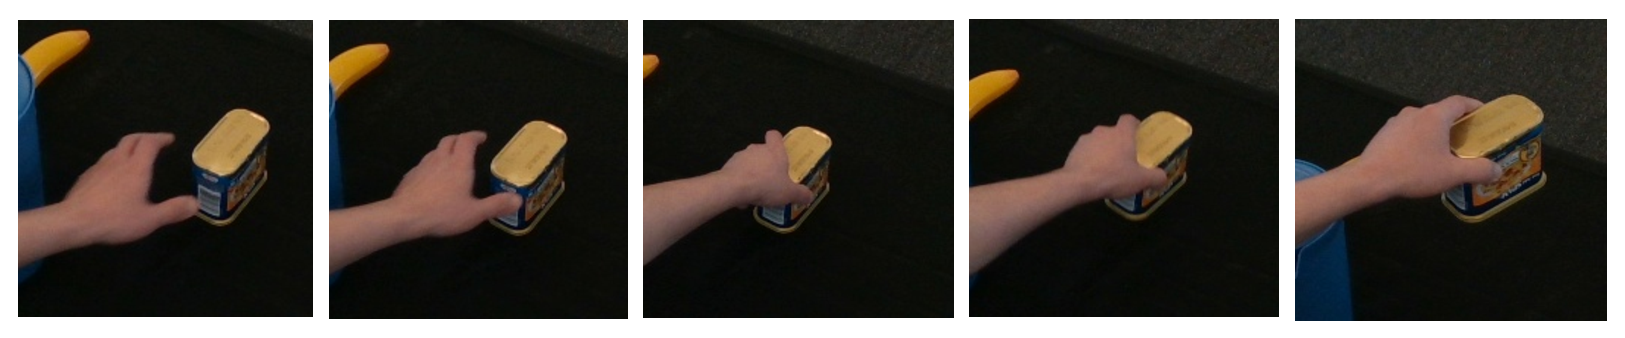
\includegraphics[width=\linewidth]{figs/1_rgb}
        \caption{Input}
    \end{subfigure}
    \hfill
    \begin{subfigure}{0.98\textwidth}
        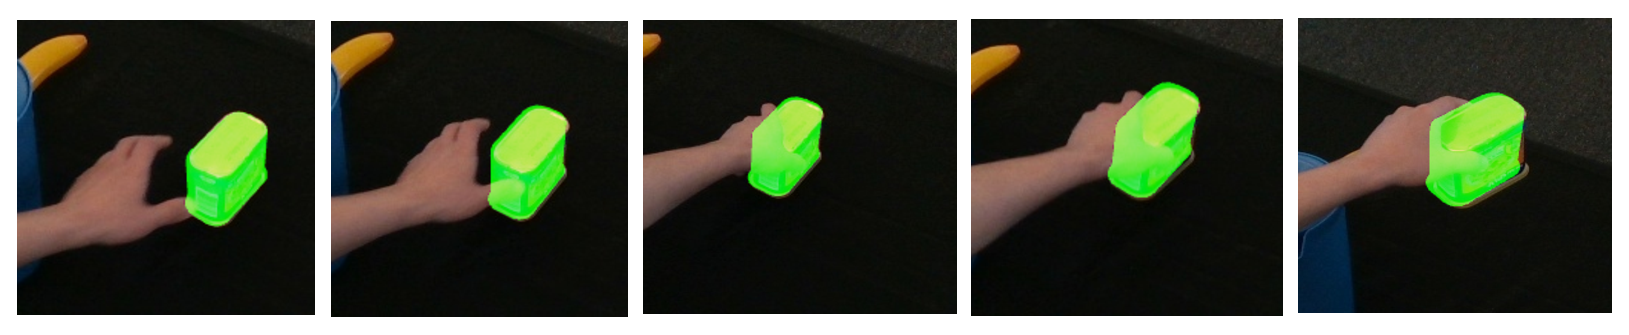
\includegraphics[width=\linewidth]{figs/1_0}
        \caption{Ground truth}
    \end{subfigure}
    \hfill
    \begin{subfigure}{0.98\textwidth}
        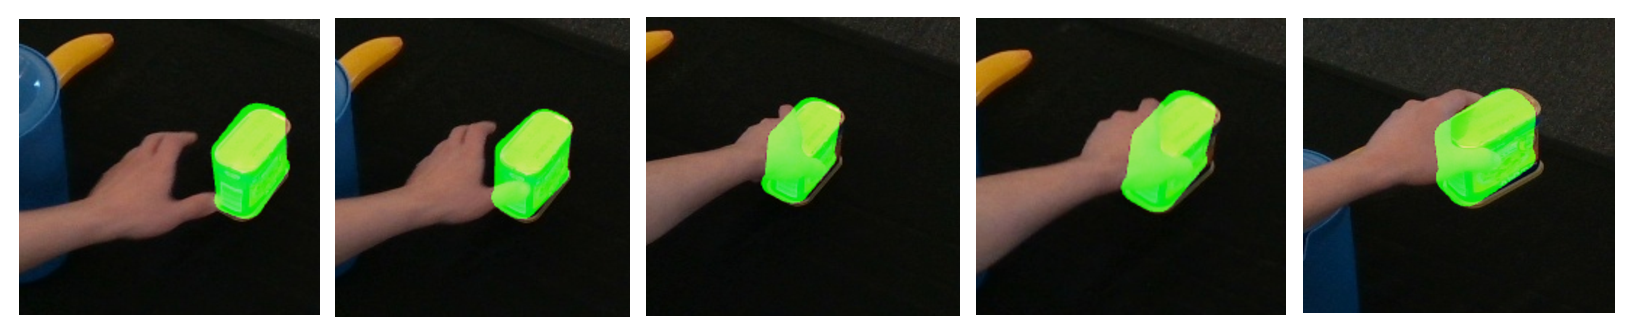
\includegraphics[width=\linewidth]{figs/1_1}
        \caption{Ours}
    \end{subfigure}
    \hfill
    \begin{subfigure}{0.98\textwidth}
        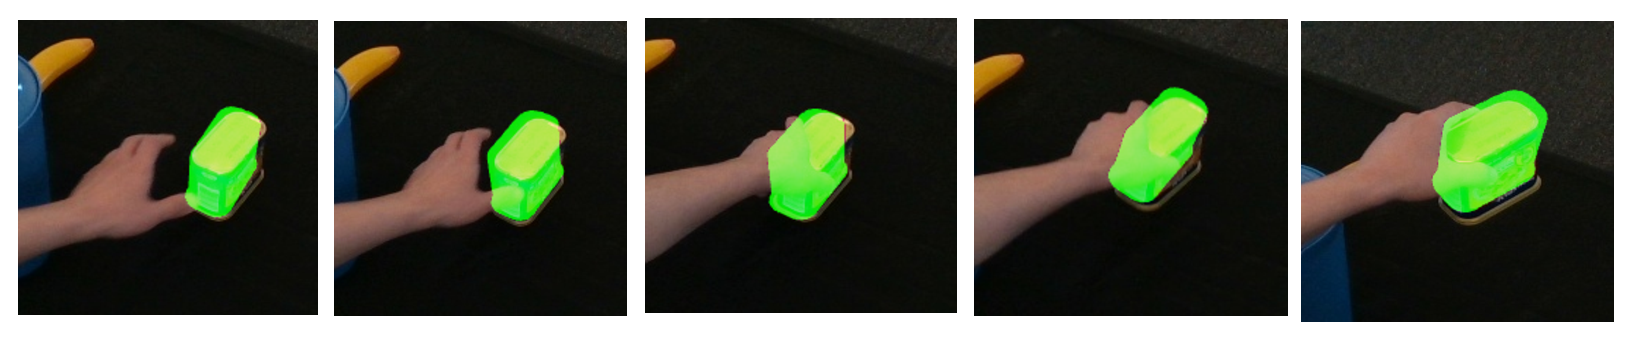
\includegraphics[width=\linewidth]{figs/1_2}
        \caption{Wang et al. \cite{wang2023deep}}
    \end{subfigure}
    \hfill
    \begin{subfigure}{0.98\textwidth}
        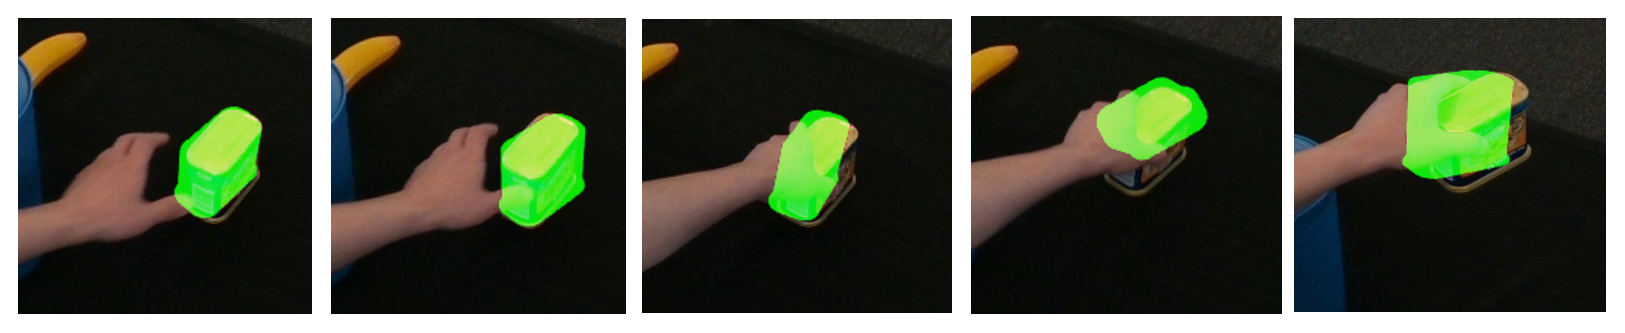
\includegraphics[width=\linewidth]{figs/1_3}
        \caption{Castro et al. \cite{castro2023crt}}
    \end{subfigure}
    \caption{Qualitative Comparison of the state-of-the-art single-view method \cite{castro2023crt}, video-based method \cite{wang2023deep},
and our method. The proposed method robustly generates more stable and accurate poses over time than previous approaches. (a) are the input RGBD images. (b) shows the rendered images using ground truth object poses. (c), (d), and (e) display the rendered images using predicted object poses.}
    \label{fig:result1}
\end{figure*}

%-------------------------------------------------------
\begin{figure*}[!ht]
    \begin{subfigure}{0.98\textwidth}
        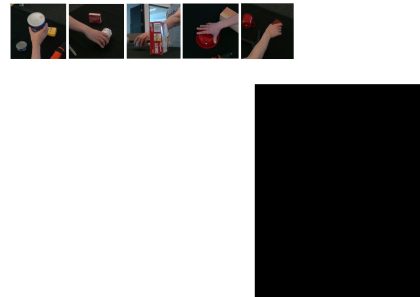
\includegraphics[width=\linewidth]{figs/2_rgb}
        \caption{Input}
    \end{subfigure}
    \hfill
    \begin{subfigure}{0.98\textwidth}
        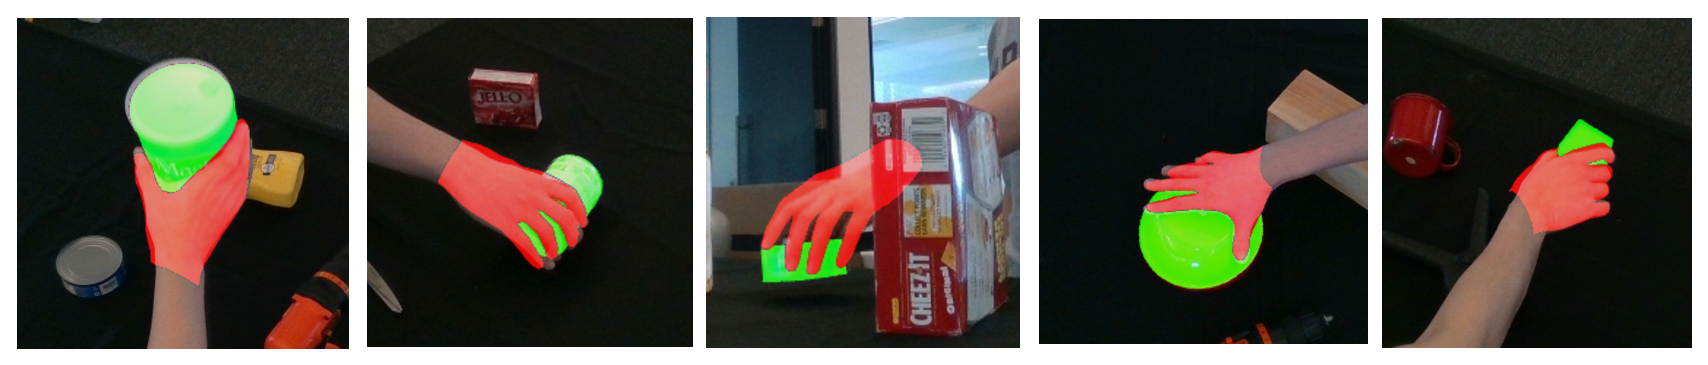
\includegraphics[width=\linewidth]{figs/2_0}
        \caption{Ground truth}
    \end{subfigure}
    \hfill
    \begin{subfigure}{0.98\textwidth}
        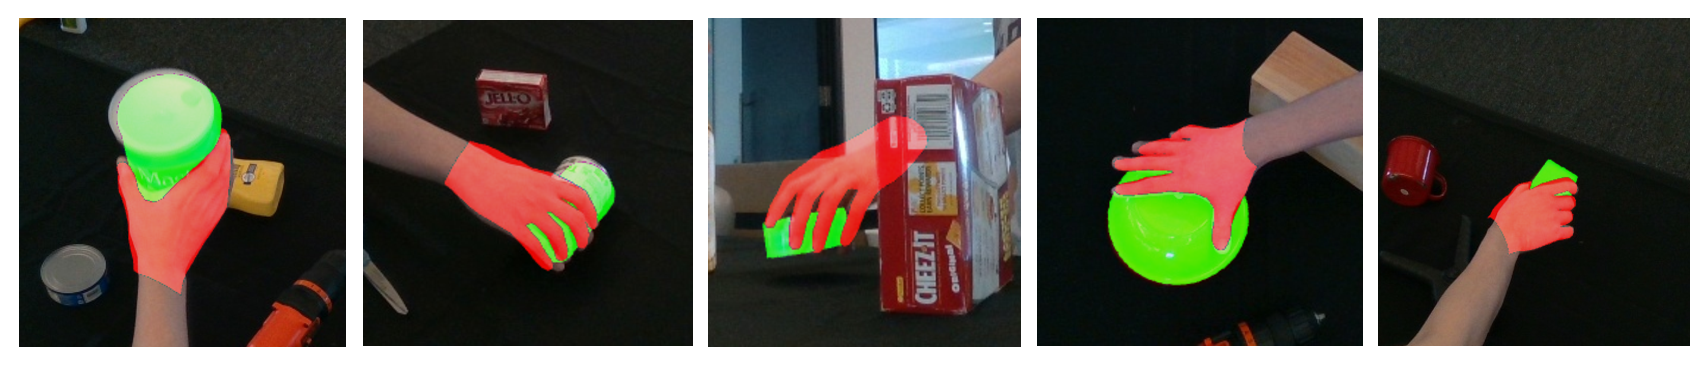
\includegraphics[width=\linewidth]{figs/2_1}
        \caption{Ours}
    \end{subfigure}
    \hfill
    \begin{subfigure}{0.98\textwidth}
        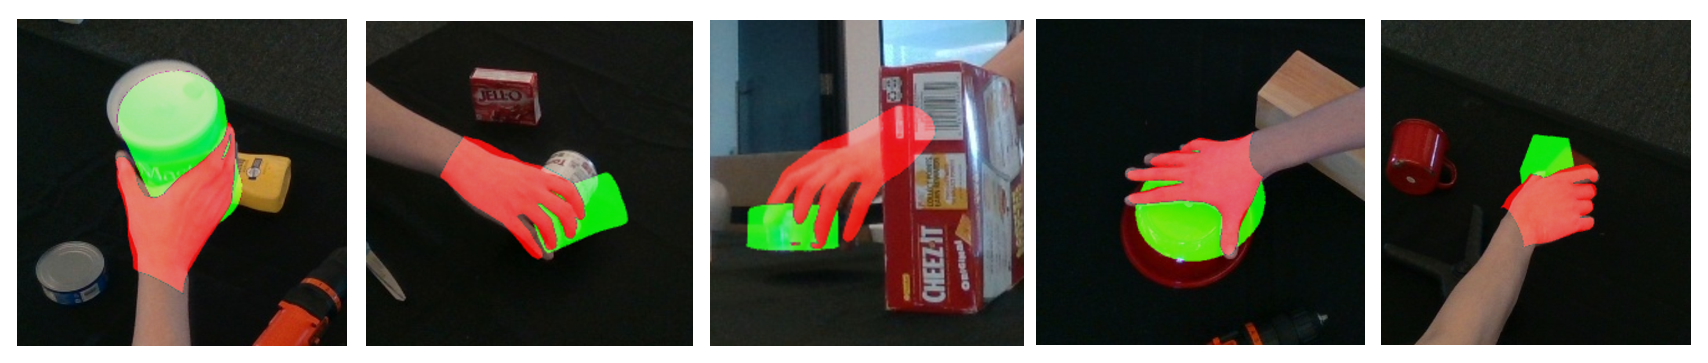
\includegraphics[width=\linewidth]{figs/2_2}
        \caption{Wang et al. \cite{wang2023deep}}
    \end{subfigure}
    \hfill
    \begin{subfigure}{0.98\textwidth}
        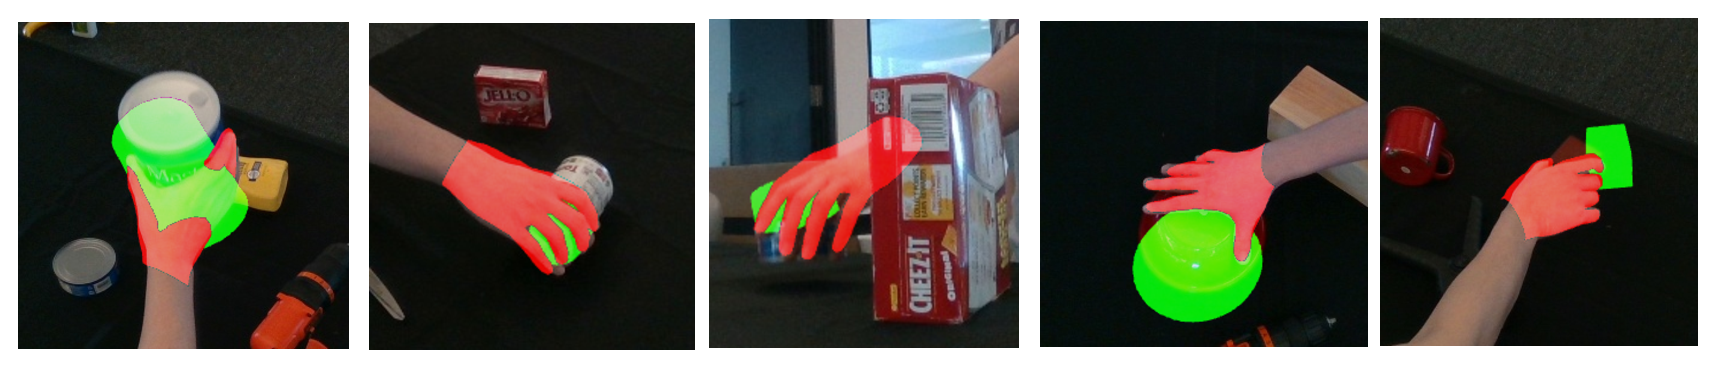
\includegraphics[width=\linewidth]{figs/2_3}
        \caption{Castro et al. \cite{castro2023crt}}
    \end{subfigure}
    \caption{Qualitative Comparison of the state-of-the-art single-view method \cite{castro2023crt}, video-based method \cite{wang2023deep},
and our method. Here we only show results on frames under heavy occlusion (frames with a visibility score \( v_i \) smaller than \( \delta = 0.5 \)). (a) are the input RGBD images. (b) shows the rendered images using ground truth hand and object poses. (c), (d), and (e) display the rendered images using ground truth hand poses and predicted object poses.}
    \label{fig:result2}
\end{figure*}
%-------------------------------------------------------

\subsection{Evaluation Metric}
\label{sec:metric}

To evaluate the accuracy of the estimated pose \(\mathbf{\hat{P}}\) compared to the ground-truth pose \(\mathbf{\bar{P}}\) of an object model \(M\), we employ Average Distance of Model Points (ADD) metric \cite{hinterstoisser2012model}. This metric determines the average distance between corresponding vertices of the object in its ground-truth and estimated poses. Mathematically, given the ground-truth rotation \(\mathbf{\bar{R}}\) and translation \(\mathbf{\bar{t}}\), and the estimated rotation \(\mathbf{\hat{R}}\) and translation \(\mathbf{\hat{t}}\), the ADD is expressed as:

\begin{equation}
ADD = \frac{1}{m} \sum_{x \in M} \parallel (\mathbf{\bar{R}}x + \mathbf{\bar{t}}) - (\mathbf{\hat{R}}x + \mathbf{\hat{t}}) \parallel,
\end{equation}

\noindent where \(m\) represents the number of points on the object model. For symmetric objects, the ADD metric is modified to use the minimum distance between corresponding points, as described in \cite{bregier2017symmetry}. We assess the accuracy of the pose predictions using the Average Precision (AP) metric \cite{bregier2017symmetry}, where a 6D pose estimate is classified as a true positive if the ADD is within 10\% of the object's smallest bounding sphere diameter. Additionally, we report the Area Under the ADD Curve (AUC) \cite{wang2019densefusion}, which summarizes the model's performance across a range of error thresholds.

\subsection{Result}

Figures \ref{fig:result1} and \ref{fig:result2} provide a qualitative comparison of the proposed method with existing state-of-the-art methods for in-hand object pose estimation. In Figure \ref{fig:result1}, the proposed method consistently produces more stable and accurate pose predictions over time compared to single-view and video-based methods. In Figure \ref{fig:result2}, the comparison focuses on frames with heavy occlusion. The visibility-aware module in our approach allows the system to leverage temporal information from neighboring frames, resulting in accurate pose estimation despite the lack of clear visual cues. Both Wang et al. and Castro et al.'s methods struggle in these scenarios, as evidenced by the distorted and less accurate object poses. Our method, by contrast, maintains reliable predictions under occlusion, demonstrating the effectiveness of integrating the visibility-aware module into the spatial-temporal architecture.

%----------------------------------------------------------
\begin{table*}[h]
\caption{Quantitative results on the DexYCB \cite{chao2021dexycb}, FPHAB \cite{garcia2018first}, and HO-3D \cite{hampali2020honnotate} datasets. Single image -based methods \cite{billings2019silhonet, peng2019pvnet, wang2021gdr, castro2023crt}, and tracking methods \cite{sun2021robust, huang2021pixel, he2021ffb6d, stoiber2020sparse, stoiber2022srt3d, tian2022large, wang2023deep} are compared with our proposed method (Ours).}
\label{tab:dataset_ex}
\begin{center}
\begin{tabular}{l c c c c c c c} 
\hline
& \multicolumn{2}{c}{DexYCB} & \multicolumn{2}{c}{FPHAB} & \multicolumn{2}{c}{HO-3D} & Time \\
\hline
Method & $AUC$ & $AP$ & $AUC$ & $AP$ & $AUC$ & $AP$ & $ms$ \\  
\hline 
Billings et al. \cite{billings2019silhonet} & 54.1 & 55.2 & 56.5 & 57.4 & 55.7 & 56.2 & 35 \\

Peng et al. \cite{peng2019pvnet} & 57.6 & 58.5 & 59.1 & 60.3 & 58.3 & 59.2 & 38 \\

Wang et al.\cite{wang2021gdr} & 59.3 & 60.8 & 61.2 & 62.6 & 60.4 & 61.4 & 32 \\

Castro et al. \cite{castro2023crt} & 61.5 & 62.4 & 63.6 & 64.3 & 62.6 & 63.7 & 30 \\

\hline 

Sun et al. \cite{sun2021robust} & 60.5 & 61.4 & 63.6 & 64.2 & 61.9 & 62.6 & 87 \\

Huang et al. \cite{huang2021pixel} & 68.3 & 69.5 & 69.5 & 70.2 & 68.1 & 69.4 & 67 \\

Stoiber et al. \cite{stoiber2020sparse} & 67.2 & 67.5 & 68.4 & 69.2 & 67.9 & 68.3 & 98 \\

Stoiber et al. \cite{stoiber2022srt3d} & 71.4 & 72.8 & 73.5 & 74.3 & 71.1 & 72.2 & 87 \\

Tian et al. \cite{tian2022large} & 72.4 & 72.9 & 74.1 & 75.4 & 73.3 & 74.2 & 78 \\

Wang et al. \cite{wang2023deep} & 74.6 & 75.5 & 76.2 & 77.1 & 76.0 & 76.3 & 33 \\

Ours & \textbf{80.1} & \textbf{80.8} & \textbf{81.6} & \textbf{82.6} & \textbf{81.1} & \textbf{82.3} & 66 \\
\hline
\end{tabular}
\end{center}
\end{table*}

%-------------------------------------------------

Table \ref{tab:dataset_ex} presents the quantitative comparison of our proposed method with both single-image-based and tracking-based methods across three datasets: DexYCB \cite{chao2021dexycb}, FPHAB \cite{garcia2018first}, and HO-3D \cite{hampali2020honnotate}. The metrics used for evaluation are AUC (Area Under the ADD Curve) and AP (Average Precision). The table clearly illustrates that single-image-based methods, such as \cite{billings2019silhonet}, \cite{peng2019pvnet}, \cite{wang2021gdr}, and \cite{castro2023crt}, underperform compared to tracking-based methods, which is expected given the importance of temporal information in in-hand object pose tracking tasks. Among the tracking-based methods, \cite{wang2023deep} delivers strong performance with AUC scores of 74.6\%, 76.2\%, and 76.0\% on the DexYCB, FPHAB, and HO-3D datasets, respectively. However, our proposed method significantly outperforms all other approaches, achieving the highest AUC scores of 80.1\%, 81.6\%, and 81.1\% across these datasets. This improvement is attributed to the incorporation of transformers for spatial-temporal modeling and the visibility-aware module, which effectively handles occlusions and maintains robust pose estimation even under challenging conditions. Additionally, our method demonstrates competitive inference time, operating at 66ms per frame. Although not the fastest, it offers a well-balanced trade-off between execution speed and performance, outperforming faster but less accurate methods such as \cite{castro2023crt} and \cite{wang2021gdr}. These results validate the effectiveness of our approach in enhancing the accuracy and robustness of in-hand object pose tracking across diverse real-world scenarios.


%----------------------------------------------------------
\begin{table*}[h]
\caption{Quantitative results on the DexYCB \cite{chao2021dexycb}, FPHAB \cite{garcia2018first}, and HO-3D \cite{hampali2020honnotate} datasets. However, here we only evaluate methods on frames under heavy occlusion (frames with a visibility score \( v_i \) smaller than \( \delta = 0.5 \)). Single image-based methods \cite{billings2019silhonet, peng2019pvnet, wang2021gdr, castro2023crt}, and tracking methods \cite{sun2021robust, huang2021pixel, he2021ffb6d, stoiber2020sparse, stoiber2022srt3d, tian2022large, wang2023deep} are compared with our proposed method (Ours).}
\label{tab:occlusion_ex}
\begin{center}
\begin{tabular}{l c c c c c c c} 
\hline
& \multicolumn{2}{c}{DexYCB } & \multicolumn{2}{c}{FPHAB } & \multicolumn{2}{c}{HO-3D} & Time \\
\hline
Method & $AUC$ & $AP$ & $AUC$ & $AP$ & $AUC$ & $AP$ & $ms$ \\  
\hline 
Billings et al. \cite{billings2019silhonet} & 48.4 & 49.6 & 51.0 & 52.3 & 50.3 & 51.5 & 35 \\

Peng et al. \cite{peng2019pvnet} & 52.1 & 53.6 & 54.5 & 56.1 & 53.0 & 54.1 & 38 \\

Wang et al. \cite{wang2021gdr} & 54.8 & 54.4 & 56.0 & 57.3 & 55.4 & 56.3 & 32 \\

Castro et al. \cite{castro2023crt} & 55.2 & 56.2 & 57.0 & 57.3 & 58.1 & 58.9 & 30 \\

\hline 

Sun et al. \cite{sun2021robust} & 58.2 & 57.1 & 60.1 & 61.2 & 60.2 & 61.3 & 87 \\

Huang et al. \cite{huang2021pixel} & 63.9 & 64.8 & 64.6 & 65.0 & 63.5 & 64.6 & 67 \\

Stoiber et al.\cite{stoiber2020sparse} & 61.1 & 61.5 & 62.6 & 63.1 & 61.4 & 62.0 & 98 \\

Stoiber et al. \cite{stoiber2022srt3d} & 63.5 & 63.9 & 64.6 & 65.1 & 66.7 & 67.0 & 87 \\

Tian et al. \cite{tian2022large} & 65.0 & 65.8 & 67.7 & 68.5 & 66.8 & 67.4 & 78 \\

Wang et al. \cite{wang2023deep} & 67.3 & 68.4 & 69.1 & 70.0 & 69.7 & 69.2 & 33 \\

Ours & \textbf{78.3} & \textbf{78.5} & \textbf{79.4} & \textbf{80.1} & \textbf{79.6} & \textbf{80.8} & 66 \\
\hline
\end{tabular}
\end{center}
\end{table*}
%-------------------------------------------------

Table \ref{tab:occlusion_ex} evaluates the performance of various methods under heavy occlusion, specifically focusing on frames with a visibility score \( v_i \) smaller than \( \delta = 0.5 \). Compared to Table \ref{tab:dataset_ex} in the previous section, which evaluates overall performance, the results here reveal a key strength of our proposed method: its robustness under challenging occlusions. While most methods experience a significant drop in performance when evaluated under heavy occlusion, our method shows only a slight reduction in accuracy. For instance, on the DexYCB dataset, our method achieves an AUC of 78.3\%, compared to 80.1\% in the general evaluation from Table \ref{tab:dataset_ex}, representing a minor 1.8\% decrease. Similarly, on the FPHAB and HO-3D datasets, our method exhibits minimal reductions in AUC, with only a 2.2\% and 1.5\% decrease, respectively. In contrast, other methods suffer more substantial performance degradation under occlusion. For example, \cite{wang2023deep}, which performed well in the general evaluation, drops from 74.6\% to 67.3\% in AUC on the DexYCB dataset, representing a 7.3\% decrease. This trend is consistent across all datasets, where competing methods see larger reductions in both AUC and AP metrics. The relative stability of our method's performance highlights the effectiveness of the proposed modules, particularly the visibility-aware object pose estimation module. By dynamically adjusting pose predictions based on the visibility of the object and aggregating information from less occluded frames, our approach significantly mitigates the impact of occlusions on pose estimation accuracy. This robustness is crucial for maintaining reliable performance in real-world applications where occlusions are common, and further underscores the importance of our hybrid architecture that integrates both spatial-temporal reasoning and visibility-aware mechanisms.

\subsection{Ablation Study}

%----------------------------------------------------------
\begin{table*}[h]
\caption{Ablation Study. $\mathcal{M}_{s}$ spatial transformer, $\mathcal{M}_{t}$ temporal transformer, $\mathcal{M}_{va}$ visibility-aware object pose estimation module.}
\label{tab:ablation_ex}
\begin{center}
\begin{tabular}{l c c c c c c c} 
\hline
& \multicolumn{2}{c}{DexYCB} & \multicolumn{2}{c}{FPHAB} & \multicolumn{2}{c}{HO-3D} & Time \\
\hline
Method & $AUC$ & $AP$ & $AUC$ & $AP$ & $AUC$ & $AP$ & $ms$ \\  
\hline 

Without Transformers & 58.2 & 57.1 & 60.1 & 61.2 & 60.2 & 61.3 & 87 \\

Without $\mathcal{M}_{t}$ and $\mathcal{M}_{s}$ & 65.7 & 66.4 & 68.5 & 68.9 & 67.2 & 68.4 & 28 \\

Without $\mathcal{M}_{s}$ & 73.7 & 74.1 & 74.2 & 75.0 & 76.3 & 77.2 & 35 \\

Without $\mathcal{M}_{t}$ & 71.2 & 72.3 & 74.9 & 76.3 & 73.5 & 74.0 & 36 \\

Without $\mathcal{M}_{va}$ & 75.1 & 77.2 & 76.5 & 76.8 & 75.6 & 76.9 & 34 \\

Ours (Full) & \textbf{80.1} & \textbf{80.8} & \textbf{81.6} & \textbf{82.6} & \textbf{81.1} & \textbf{82.3} & 66 \\
\hline
\end{tabular}
\end{center}
\end{table*}

%-------------------------------------------------

Table \ref{tab:ablation_ex} presents the results of the ablation study, which evaluates the contributions of the spatial transformer module ($\mathcal{M}_{s}$), temporal transformer module ($\mathcal{M}_{t}$), and visibility-aware object pose estimation module ($\mathcal{M}_{va}$) to the overall performance of our proposed method. The goal of this analysis is to assess the impact of each component by systematically removing them from the model and measuring the resulting performance on the DexYCB, FPHAB, and HO-3D datasets.

The results show that removing either the spatial or temporal transformers leads to a significant drop in performance. For instance, when both $\mathcal{M}_{s}$ and $\mathcal{M}_{t}$ are excluded, the AUC drops to 65.7\% on DexYCB, indicating a substantial decrease of 14.4\% compared to the full model. This highlights the importance of spatial-temporal reasoning for capturing the dynamic nature of in-hand object pose tracking. Similarly, removing only the spatial transformer ($\mathcal{M}_{s}$) results in a notable performance drop, with an AUC of 73.7\% on DexYCB, which underscores the critical role that spatial dependencies play in enhancing the model's understanding of object-hand interactions within individual frames. When the temporal transformer ($\mathcal{M}_{t}$) is excluded, the model also suffers a decline in performance across all datasets. For example, on the HO-3D dataset, the AUC decreases from 81.1\% (full model) to 73.5\%, demonstrating the essential role of temporal reasoning in improving pose estimation accuracy across video sequences. This result indicates that while spatial information is crucial, temporal dependencies are equally important for maintaining robust tracking performance over time. The visibility-aware module ($\mathcal{M}_{va}$) also plays a significant role in handling occlusions. Removing this module results in a moderate drop in performance, with the AUC on DexYCB decreasing to 75.1\%. This reduction in accuracy highlights the effectiveness of the visibility-aware mechanism in ensuring reliable pose estimation even in frames where the object is partially or fully occluded. By dynamically adjusting predictions based on object visibility and aggregating information from neighboring frames, this module enhances the model's robustness in challenging scenarios. Overall, the ablation study confirms that the combination of the spatial transformer, temporal transformer, and visibility-aware modules is critical for achieving the best performance. The full model consistently outperforms its ablated variants across all datasets, with an AUC of 80.1\% on DexYCB, 81.6\% on FPHAB, and 81.1\% on HO-3D. Despite the added complexity of integrating these components, the inference time remains competitive at 66ms, demonstrating that the proposed method offers a practical balance between accuracy and efficiency for real-time in-hand object pose tracking applications.

\section{Conclusion}

In this paper, we introduced a novel framework for in-hand object pose tracking that effectively addresses the challenges posed by dynamic occlusions and rapid hand movements. By leveraging a hybrid architecture that combines the strengths of convolutional neural networks (CNNs) for spatial feature extraction with transformers for temporal reasoning, our method achieves robust and accurate pose estimation across video sequences. A key innovation of our approach is the visibility-aware module, which dynamically adjusts pose predictions based on the object's visibility, allowing the model to maintain high accuracy even under challenging conditions where portions of the object are occluded or blurred. Extensive experiments conducted on three public datasets DexYCB, FPHAB, and HO-3D demonstrate the superior performance of our method compared to existing state-of-the-art techniques. Our approach consistently outperforms these methods across various metrics, highlighting its effectiveness in both standard and occlusion-heavy scenarios. The results of the ablation studies further validate the importance of each component in our model, particularly the integration of spatial-temporal transformers and the visibility-aware mechanism, which collectively contribute to the robustness and accuracy of the pose tracking process.

Beyond achieving competitive accuracy, our method also maintains a practical balance between performance and computational efficiency, making it suitable for real-time applications in fields such as robotics, augmented reality, and human-computer interaction. The ability to accurately track objects in-hand, even under challenging conditions, opens up new possibilities for enhancing the interactivity and functionality of systems in these domains. For future work, we plan to explore the extension of our framework to handle more complex and cluttered environments, as well as its application to multi-object pose tracking scenarios. Additionally, we aim to optimize the computational aspects of our model further, enabling faster inference while preserving accuracy, thereby enhancing its applicability to real-time, resource-constrained environments. By continuing to refine and expand our approach, we hope to contribute to the development of more intelligent and adaptive systems capable of understanding and interacting with the physical world in a more sophisticated manner. \\


%
\bibliographystyle{IEEEtran}
\bibliography{References}

\begin{IEEEbiography}[{\includegraphics[width=1in,height=1.25in,clip,keepaspectratio]{authors/prof_Tan}}]{Phan Xuan Tan} (Member, IEEE) received the B.E. degree in Electrical-Electronic Engineering from Military Technical Academy, Vietnam, M.E. degree in Computer and Communication Engineering from Hanoi University of Science and Technology, Vietnam and Ph.D. degree in Functional Control Systems from Shibaura Institute of Technology, Japan. He is currently an Associate Professor at Shibaura Institute of Technology. His current research interests include computer vision, deep learning and image processing.
\end{IEEEbiography}

\begin{IEEEbiography}[{\includegraphics[width=1in,height=1.25in,clip,keepaspectratio]{authors/DinhCuong}}]{Dinh-Cuong Hoang} received his Ph.D. degree in computer science from Orebro University, Sweden (2021), and is currently a lecturer at FPT University, Greenwich Vietnam. His research interests lie at the intersection of computer vision, robotics, and machine learning. He is particularly interested in topics involving autonomy for robots, with a focus on perception algorithms.
\end{IEEEbiography}

\begin{IEEEbiography}[{\includegraphics[width=1in,height=1.25in,clip,keepaspectratio]{authors/Eiji_Kamioka}}]{Eiji Kamioka} (Member, IEEE) received the B.S., M.S., and D.S. degrees in physics from Aoyama Gakuin University. He is a Professor with the Shibaura Institute of Technology (SIT). Before joining the SIT, he was working with the SHARP Communication Laboratory, Institute of Space and Astronautical Science (ISAS), as a JPSP Research Fellow, and the National Institute of Informatics (NII) as an Assistant Professor. His current research interests encompass mobile multimedia communications and ubiquitous computing.
\end{IEEEbiography}

\begin{IEEEbiography}[{\includegraphics[width=1in,height=1.25in,clip,keepaspectratio]{authors/NguyenAnhNhat}}]{Anh-Nhat Nguyen}  is currently a lecturer at FPT University, Vietnam. He received his B.S. and M.S. degrees in Computer Science from Duy Tan University, Da Nang, Vietnam, in 2012 and from Huazhong University of Science and Technology (HUST), China, in 2018, respectively. His research interests include image processing, information security, physical layer secrecy, radio-frequency energy harvesting, and wireless sensor networks.
\end{IEEEbiography}

\begin{IEEEbiography}[{\includegraphics[width=1in,height=1.25in,clip,keepaspectratio]{authors/TranDucThanh}}]{Duc-Thanh Tran} is pursuing a B.S. degree in Artificial Intelligence at FPT University, Hanoi, Vietnam, with a primary focus on research in the field of computer vision.
\end{IEEEbiography}

\begin{IEEEbiography}[{\includegraphics[width=1in,height=1.25in,clip,keepaspectratio]{authors/DuongVanHiep}}]{Van-Hiep Duong} is pursuing a B.S. degree in Artificial Intelligence at FPT University, Hanoi, Vietnam, with a primary focus on research in the field of computer vision.
\end{IEEEbiography}

\begin{IEEEbiography}[{\includegraphics[width=1in,height=1.25in,clip,keepaspectratio]{authors/MaiAnhTruong}}]{Anh-Truong Mai} is pursuing a B.S. degree in Artificial Intelligence at FPT University, Hanoi, Vietnam, with a primary focus on research in the field of computer vision.
\end{IEEEbiography}

\begin{IEEEbiography}[{\includegraphics[width=1in,height=1.25in,clip,keepaspectratio]{authors/PhamDucLong}}]{Duc-Long Pham} is pursuing a B.S. degree in Artificial Intelligence at FPT University, Hanoi, Vietnam, with a primary focus on research in the field of computer vision.
\end{IEEEbiography}

\begin{IEEEbiography}[{\includegraphics[width=1in,height=1.25in,clip,keepaspectratio]{authors/PhanKhanhToan}}]{Khanh-Toan Phan} is pursuing a B.S. degree in Artificial Intelligence at FPT University, Hanoi, Vietnam, with a primary focus on research in the field of computer vision.
\end{IEEEbiography}

\begin{IEEEbiography}[{\includegraphics[width=1in,height=1.25in,clip,keepaspectratio]{authors/DuongVanHiep}}]{Van-Hiep Duong} is pursuing a B.S. degree in Artificial Intelligence at FPT University, Hanoi, Vietnam, with a primary focus on research in the field of computer vision.
\end{IEEEbiography}

\begin{IEEEbiography}[{\includegraphics[width=1in,height=1.25in,clip,keepaspectratio]{authors/DinhXuanTung}}]{Xuan-Tung Dinh} is pursuing a B.S. degree in Artificial Intelligence at FPT University, Hanoi, Vietnam, with a primary focus on research in the field of computer vision.
\end{IEEEbiography}

\begin{IEEEbiography}[{\includegraphics[width=1in,height=1.25in,clip,keepaspectratio]{authors/TranThiThuyTrang}}]{TranThiThuyTrang} is pursuing a B.S. degree in Information Technology at FPT University, Hanoi, Vietnam.
\end{IEEEbiography}

\begin{IEEEbiography}[{\includegraphics[width=1in,height=1.25in,clip,keepaspectratio]{authors/PhamXuanDuong}}]{Xuan-Duong Pham} is pursuing a B.S. degree in Information Technology at FPT University, Hanoi, Vietnam.
\end{IEEEbiography}

\begin{IEEEbiography}[{\includegraphics[width=1in,height=1.25in,clip,keepaspectratio]{authors/NguyenNhatLinh}}]{Nhat-Linh Nguyen} is pursuing a B.S. degree in Information Technology at FPT University, Hanoi, Vietnam.
\end{IEEEbiography}

\begin{IEEEbiography}[{\includegraphics[width=1in,height=1.25in,clip,keepaspectratio]{authors/TrinhVietAnh}}]{Viet-Anh Trinh} is pursuing a B.S. degree in Information Technology at Greenwich Vietnam, FPT University, Hanoi, Vietnam.
\end{IEEEbiography}

\begin{IEEEbiography}[{\includegraphics[width=1in,height=1.25in,clip,keepaspectratio]{authors/TranKhanhDuong}}]{Khanh-Duong Tran} is pursuing a B.S. degree in Information Technology at Greenwich Vietnam, FPT University, Hanoi, Vietnam.
\end{IEEEbiography}

\begin{IEEEbiography}[{\includegraphics[width=1in,height=1.25in,clip,keepaspectratio]{authors/BuiSonAnh}}]{Son-Anh Bui} is pursuing a B.S. degree in Information Technology at Greenwich Vietnam, FPT University, Hanoi, Vietnam.
\end{IEEEbiography}

\EOD

\end{document}
